% Deep Learning - Milestone 1 (max ~3 pages body; compile with: pdflatex, bibtex, pdflatex x2)
% Optional: replace document class with CVPR/NeurIPS author kit from https://github.com/cvpr-org/author-kit/releases
\documentclass[10pt,a4paper]{article}
\usepackage[utf8]{inputenc}
\usepackage[T1]{fontenc}
\usepackage{lmodern}
\usepackage[margin=1.65cm]{geometry}
\usepackage{microtype,graphicx,booktabs,hyperref}
\usepackage{amsmath,amssymb}
\usepackage[numbers,sort&compress]{natbib}
\usepackage{tikz}
\usetikzlibrary{arrows.meta,positioning}
\setlength{\parindent}{0pt}
\setlength{\parskip}{0.4em}
\newcommand{\kteam}{Thalia Delhaise (66937), Lenny Briclet (66926), Andr\'e Fonseca (58225), Rafael Gufler (66081)}

\title{FB15k-237 Link Prediction: Baseline Training and Preliminary Experiments}
\author{\kteam}
\date{Project 425282 --- Report for Milestone 1 (Deep Learning)}

\begin{document}
\maketitle
\thispagestyle{empty}
\vspace{-0.6em}
\begin{abstract}
We build the multi-relational \textbf{FB15k-237} graph, train classical knowledge graph embedding baselines \textbf{TransE} and \textbf{RotatE} with the same splits and \textbf{filtered} ranking protocol, and report preliminary \textbf{MRR / Hits@k} with training curves. This report covers the \textbf{data pipeline}, the \textbf{baseline} setup, \textbf{known issues}, and a plan for the remaining experiments: custom hard negatives, slice metrics, and a small relational GNN, each with ablations. For a shorter topic outline (Milestone~0) see the one-page project proposal. Code: \texttt{code/train\_baseline\_kge.py} in the repository; optional CVPR/NeurIPS template can be swapped in for the final version.
\end{abstract}

\subsection*{1.\ Introduction and plan}
\emph{Goal:} given training triples $(h,r,t)$ in a knowledge graph, rank the correct missing entity for queries $(h,r,?)$ and $(?,r,t)$. We compare \textsc{TransE} to the stronger \textsc{RotatE}~\citep{sun2019rotate} on \textbf{identical} train/val/test partitions and the same \textbf{filtered} evaluation (true triples in any split are not treated as false tails/heads) per~\citet{bordes2013translating}. The overall scientific question (post feedback) is: \emph{where} improvements appear---aggregate vs.\ relation- or degree-specific regimes---and whether later \textbf{custom} negative mining and a \textbf{GNN} change that picture. Milestone~1 must show \textbf{data ready}, a \textbf{baseline} running end-to-end, \textbf{preliminary} metrics and curves, and a clear \textbf{next-step} plan.

\subsection*{2.\ Problem statement, dataset, and evaluation}
\textbf{Dataset.} \textbf{FB15k-237:} 14,541 entities, 237 relations, 272,115 / 17,535 / 20,466 train, validation, and test triples (official split)~\citep{sun2019rotate}. The graph is $\mathcal{G}=(\mathcal{E},\mathcal{R},\mathcal{T})$, $\mathcal{T}\subseteq\mathcal{E}\times\mathcal{R}\times\mathcal{E}$. No extra subsampling.

\textbf{Metrics.} \textbf{Filtered} mean reciprocal rank (MRR) and Hits@$k$ ($k\in\{1,3,10\}$) on head and tail prediction, then averaged, as in standard benchmarks.

\textbf{Expected.} A controlled comparison under matched hyperparameters: same embedding size $d$, same optimizer family, same maximum epochs (with early stopping on val MRR), and same number of corruptions per positive where applicable.

\subsection*{3.\ Data pipeline and preprocessing}
\textbf{Download.} The benchmark is loaded via \textbf{PyKEEN}~\citep{ali2021pykeen} (dataset name \texttt{fb15k237}, cached locally on first use). The library maps each entity and relation to integer IDs and materializes a \texttt{TriplesFactory} for train, validation, and test.

\textbf{Check.} We verify triple counts and disjointness of test from train. For Milestone~1, we will add simple \textbf{statistics} (to appear in the next version / Milestone~2): histogram of \textbf{relation} frequency and of entity \textbf{in-degree} / out-degree, plus one example each of a roughly one-to-many and many-to-one pattern for qualitative discussion.

\subsection*{4.\ Baseline models and training setup (PyKEEN)}
We start with two classical models with fixed scoring: \textsc{TransE} and \textsc{RotatE}~\citep{sun2019rotate}. The rest of this section is the \textbf{configuration we actually run} (edit \texttt{train\_baseline\_kge.py} if you change it).

\noindent\small
\begin{tabular}{@{}p{0.22\linewidth}p{0.72\linewidth}@{}}
\textbf{Model} & TransE, RotatE (separate runs) \\
\textbf{Formulation} & Entity embeddings in $\mathbb{R}^d$; score triples; rank tails/heads. \\
\textbf{Input / shape} & Mini-batch of triple indices; shape \texttt{[batch, 3]}. \\
\textbf{Negatives} & Corrupt head or tail; Bernoulli as in KGE default practice. \\
\textbf{Loss} & Margin / pairwise ranking (default per model in PyKEEN). \\
\textbf{Optimiser} & Adam or AdamW; small weight decay. \\
\textbf{Hyperparam.} & $d=128$; up to 50 epochs; \texttt{batch\_size}=512; LR $10^{-3}$; early stop if val MRR flat 10 epochs. \\
\textbf{Seed / env.} & \texttt{random\_seed=42}; Python~3, PyTorch, PyKEEN; GPU optional. \\
\textbf{Time budget} & (fill wall-clock after run) \\
\end{tabular}
\normalsize

The script writes \texttt{artifacts/baseline/<Model>\_summary.txt} and a PyKEEN result folder; copy key metrics and loss curves from the run into the table and figure above.

\begin{figure}[h]
\centering
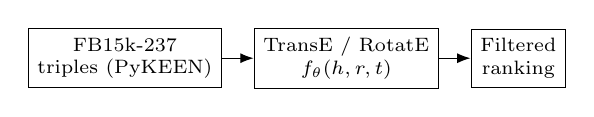
\begin{tikzpicture}[node distance=0.4cm, font=\scriptsize, >=Latex]
\node[draw,align=center] (D) {FB15k-237\\triples (PyKEEN)};
\node[draw,right=of D,align=center] (M) {TransE / RotatE\\$f_\theta(h,r,t)$};
\node[draw,right=of M,align=center] (E) {Filtered\\ranking};
\path[->] (D) edge (M) (M) edge (E);
\end{tikzpicture}
\caption{Baseline KGE data flow for Milestone~1. Later work adds a custom neg.\ sampler, slice evaluation, and a separate GNN pipeline.}
\label{fig:pipe}
\end{figure}

\subsection*{5.\ Preliminary results and training curves}
\emph{Fill in after you run the baseline script.} The table and figure below are \textbf{placeholders}; replace with real numbers and plots (PNG/PDF) exported from the training log or TensorBoard/CSV.

\begin{table}[h]
\centering
\small
\caption{Preliminary filtered metrics on the test set (replace with your run).}
\begin{tabular}{@{}lccccc@{}}
\toprule
Model & MRR & H@1 & H@3 & H@10 & Notes \\
\midrule
TransE & \textit{TBD} & \textit{TBD} & \textit{TBD} & \textit{TBD} & same $d$, budget \\
RotatE & \textit{TBD} & \textit{TBD} & \textit{TBD} & \textit{TBD} & idem \\
\bottomrule
\end{tabular}
\end{table}

\begin{figure}[h]
\centering
\begin{minipage}{0.88\linewidth}
\centering
\fbox{\rule{0pt}{1.0cm}\rule{0.92\linewidth}{0.4pt}}\\[0.3em]
\small Insert training loss and validation MRR vs.\ epoch (e.g.\ from PyKEEN log or CSV).
\end{minipage}
\caption{Placeholder for training/validation curves.}
\end{figure}

\subsection*{6.\ Known issues and next steps}
\textbf{Current issues.} (1)~Final hyperparameters may need tuning. (2)~Default negative sampling is uniform/Bernoulli: \textbf{custom} hard negative mining (separate \textbf{PyTorch} code) and ablation are planned, not in this deliverable. (3)~GNN (e.g.\ R-GCN~\citep{schlichtkrull2018modeling}) in PyG/DGL is not yet in the same repo path.

\textbf{Milestone~2 and project plan.} (a)~Relation- and degree-\textbf{slice} metrics. (b)~Error analysis: sample successes/failures by relation. (c)~Ablations: neg.\ sampling, optional $d$ and training budget. (d)~GNN on same split for comparison. (e)~Short discussion of \textbf{compute} vs.\ accuracy. Code organisation: one script per experiment family; one notebook (optional) for tables and plots.

\paragraph{Milestone~1 deliverables checklist.} \checkmark\ Data available via PyKEEN; \checkmark\ ID mappings; \checkmark\ baseline \textbf{model + architecture + loss + optim + budget} documented; \checkmark\ skeleton + runnable training script; \checkmark\ preliminary \textbf{results} (fill TBD) and curve placeholders; \checkmark\ this report; $\square$\ \textbf{fill in} actual metrics and GPU time before upload.

\paragraph{Code repository.} Baseline training: \texttt{code/train\_baseline\_kge.py}. Unify with KG course: same dataset and protocol.

\footnotesize
\bibliographystyle{plainnat}
\bibliography{../../shared/references}
\end{document}
